\section{PageRank：把网页排序变成平稳概率}
\label{sec:06-Random-Processes/04-Applications/03}

早期搜索引擎按关键词出现的频率排序。这个规则有个显而易见的后果：把``机票''这个词在页面底部用白色字体重复三百遍，你就排到了第一。凡是作者能单方面控制的信号，最终都会被作者用光。

改用链接就好一些：别人指向你，这是你自己写不出来的。可单纯数入链数量同样能刷——注册一万个空壳站点，全部指向自己。于是需要一条更严的要求：指向你的人本身也得重要。

这句话是循环的。A 的重要性取决于 C 的重要性，C 的重要性又可能取决于 A。循环定义在逻辑上是毛病，在数学上却常常是方程。PageRank 做的就是把它读成一个方程，而且是一个我们上一单元已经解过的方程。

\subsection{把重要性定义成长期访问频率}

设想一个不带任何偏好的浏览者：他停在某一页，从这一页的所有出链里等概率挑一条，跳过去，再挑一条。若网页 \(i\) 的出度为 \(d_i\)，这就是转移矩阵

\[
P_{ij}=\begin{cases}1/d_i,&i\to j,\\[2pt]0,&\text{否则}.\end{cases}
\]

问长期看他有多大比例的时间停在页面 \(j\)，就是问这条 Markov 链的平稳分布。``重要性''于是有了一个可计算的定义：\(\pi_j\)。

这个定义自动把``指向你的人也得重要''装了进去。平稳方程 \(\pi_j=\sum_i\pi_iP_{ij}\) 写开就是：\(j\) 的分数等于所有指向它的页面各自把自己的分数按出度均分之后送过来的总和。一个高分页面若只有一条出链，这条链就很值钱；若它指向一千个地方，每份就稀薄了。空壳站点互指没用，因为它们自己的分数本来就低。

麻烦在于，这条链的平稳分布不一定存在、不一定唯一、也不一定能被迭代找到。

\subsection{真实链接图会以三种方式破坏平稳分布}

\begin{center}
\begin{tikzpicture}[x=1cm,y=1cm,font=\small,>=stealth]
  \node[draw=black!55,circle,minimum size=0.7cm,inner sep=0pt,fill=blue!8] (a1) at (0,1.4) {\(A\)};
  \node[draw=black!55,circle,minimum size=0.7cm,inner sep=0pt,fill=blue!8] (a2) at (1.6,1.4) {\(B\)};
  \node[draw=black!55,circle,minimum size=0.7cm,inner sep=0pt,fill=red!12] (a3) at (0.8,0.1) {\(X\)};
  \draw[->,black!60] (a1) -- (a2);
  \draw[->,black!60] (a2) -- (a3);
  \draw[->,black!60] (a1) -- (a3);
  \node[align=center,font=\footnotesize,black!70] at (0.8,-1.0) {悬挂节点\\\(X\) 没有出链，\\这一行无法归一化};
  \draw[black!25] (3.2,-1.9) -- (3.2,2.3);
  \begin{scope}[shift={(4.3,0)}]
    \node[draw=black!55,circle,minimum size=0.7cm,inner sep=0pt,fill=blue!8] (b1) at (0,1.4) {\(A\)};
    \node[draw=black!55,circle,minimum size=0.7cm,inner sep=0pt,fill=red!12] (b2) at (1.5,1.4) {\(U\)};
    \node[draw=black!55,circle,minimum size=0.7cm,inner sep=0pt,fill=red!12] (b3) at (1.5,0.1) {\(V\)};
    \draw[->,black!60] (b1) -- (b2);
    \draw[->,black!60] (b2) to[bend left=18] (b3);
    \draw[->,black!60] (b3) to[bend left=18] (b2);
    \node[align=center,font=\footnotesize,black!70] at (0.9,-1.0) {蜘蛛陷阱\\进了 \(\set{U,V}\) 就出不来，\\全部质量最终堆在里面};
  \end{scope}
  \draw[black!25] (7.9,-1.9) -- (7.9,2.3);
  \begin{scope}[shift={(9.0,0)}]
    \node[draw=black!55,circle,minimum size=0.7cm,inner sep=0pt,fill=blue!8] (c1) at (0.2,1.5) {\(A\)};
    \node[draw=black!55,circle,minimum size=0.7cm,inner sep=0pt,fill=blue!8] (c2) at (1.7,1.5) {\(B\)};
    \node[draw=black!55,circle,minimum size=0.7cm,inner sep=0pt,fill=blue!8] (c3) at (0.95,0.2) {\(C\)};
    \draw[->,black!60] (c1) -- (c2);
    \draw[->,black!60] (c2) -- (c3);
    \draw[->,black!60] (c3) -- (c1);
    \node[align=center,font=\footnotesize,black!70] at (0.95,-1.0) {周期结构\\分布按周期 \(3\) 循环，\\逐时刻不收敛};
  \end{scope}
\end{tikzpicture}

\emph{三种结构各自破坏一个前提。左边连转移矩阵都写不完整；中间的链可约，平稳分布不唯一，而且答案完全由起点决定；右边不可约但有周期，方程有唯一解，迭代却永远绕着它转。这些都不是数值算法的小毛病，是链的结构问题。}
\end{center}

对照上一单元的收敛定理就能看出这三张图分别踩了哪一条。不可约保证唯一性，非周期保证逐时刻收敛，两者缺一不可（见\hyperref[sec:06-Random-Processes/03-Markov-Chains/04]{``平稳分布、可逆性与遍历收敛''}）；而蜘蛛陷阱就是\hyperref[sec:06-Random-Processes/03-Markov-Chains/02]{``可达、通信类与周期性''}里说的闭通信类，进得去出不来。真实的网页图上，这三种情形不是罕见的病例，而是随处可见的常态。

\subsection{阻尼因子买的是不可约与非周期}

修补的办法出人意料地粗暴：允许浏览者随时放弃当前页面，直接在地址栏里敲一个新地址。取 \(0<\alpha<1\) 和一个处处为正的分布 \(v\)，每一步以概率 \(\alpha\) 沿链接走，以概率 \(1-\alpha\) 按 \(v\) 随机跳。转移矩阵成为

\[
G=\alpha P+(1-\alpha)\ind v,
\]

其中 \(\ind\) 是全一列向量，所以 \(\ind v\) 的每一行都等于 \(v\)。这就是所谓的 Google 矩阵。

两个前提一次到手。从任意页面出发，一步之内到任意页面的概率至少是 \((1-\alpha)v_j>0\)，所以 \(G\) 处处为正，当然不可约；同理 \(G_{ii}>0\)，自环存在，周期只能是一。收敛定理的条件齐了：唯一的 \(\pi\) 存在，每个分量为正，且从任何初始分布迭代都收敛到它。悬挂节点单独处理，通常把它那一行整个换成 \(v\)，相当于走进死胡同就重新跳转。

值得停一下的是这个修补的性质。它没有对链接结构做任何``修正''或``清洗''，而是往图上均匀掺了一点噪声，把原本可能断裂的连通性强行补齐。为随机过程加入小概率重启从而买到遍历性，是一个到处都能复用的动作——模拟退火里的随机重启、\(\varepsilon\)-贪心里的随机探索、MCMC 里的独立提议，做的都是同一件事。

\subsection{一个四页的例子}

\begin{center}
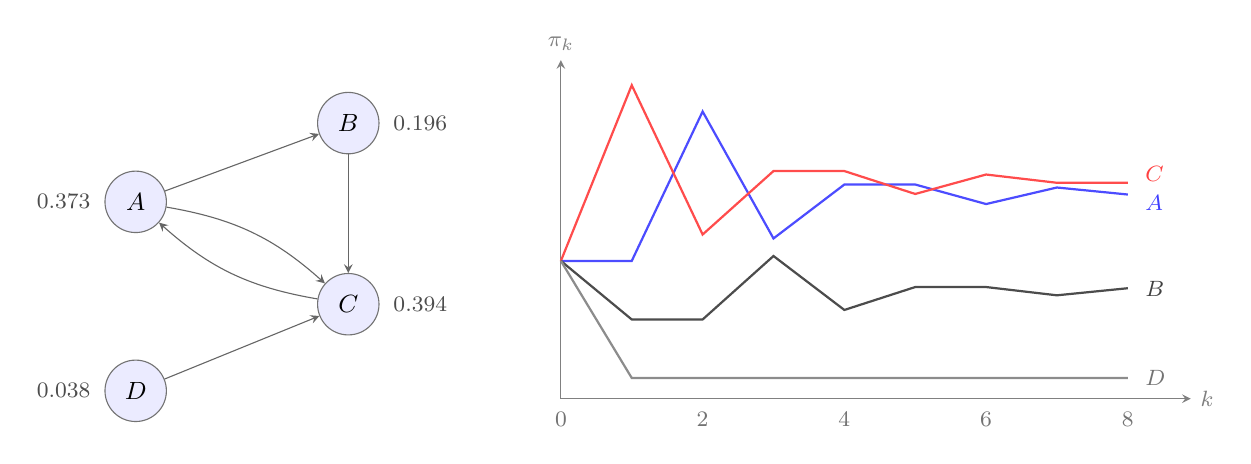
\begin{tikzpicture}[x=1cm,y=1cm,font=\small,>=stealth]
  \node[draw=black!55,circle,minimum size=0.78cm,inner sep=0pt,fill=blue!8] (A) at (0.6,1.9) {\(A\)};
  \node[draw=black!55,circle,minimum size=0.78cm,inner sep=0pt,fill=blue!8] (B) at (3.3,2.9) {\(B\)};
  \node[draw=black!55,circle,minimum size=0.78cm,inner sep=0pt,fill=blue!8] (C) at (3.3,0.6) {\(C\)};
  \node[draw=black!55,circle,minimum size=0.78cm,inner sep=0pt,fill=blue!8] (D) at (0.6,-0.5) {\(D\)};
  \draw[->,black!60] (A) -- (B);
  \draw[->,black!60] (B) -- (C);
  \draw[->,black!60] (D) -- (C);
  \draw[->,black!60] (A) to[bend left=16] (C);
  \draw[->,black!60] (C) to[bend left=16] (A);
  \node[left,font=\footnotesize,black!70] at (0.15,1.9) {\(0.373\)};
  \node[right,font=\footnotesize,black!70] at (3.75,2.9) {\(0.196\)};
  \node[right,font=\footnotesize,black!70] at (3.75,0.6) {\(0.394\)};
  \node[left,font=\footnotesize,black!70] at (0.15,-0.5) {\(0.038\)};
  \begin{scope}[shift={(6.0,-0.6)}]
    \draw[->,black!50] (0,0) -- (8.0,0) node[right,font=\footnotesize] {\(k\)};
    \draw[->,black!50] (0,0) -- (0,4.3) node[above,font=\footnotesize] {\(\pi_k\)};
    \foreach \k/\x in {0/0,2/1.8,4/3.6,6/5.4,8/7.2}
      \node[below,font=\footnotesize,black!55] at (\x,-0.05) {\k};
    \draw[blue!70,thick] (0,1.750) -- (0.9,1.750) -- (1.8,3.647) -- (2.7,2.035) -- (3.6,2.720) -- (4.5,2.720) -- (5.4,2.472) -- (6.3,2.682) -- (7.2,2.593);
    \draw[red!70,thick] (0,1.750) -- (0.9,3.981) -- (1.8,2.085) -- (2.7,2.891) -- (3.6,2.891) -- (4.5,2.600) -- (5.4,2.847) -- (6.3,2.742) -- (7.2,2.742);
    \draw[black!70,thick] (0,1.750) -- (0.9,1.006) -- (1.8,1.006) -- (2.7,1.812) -- (3.6,1.127) -- (4.5,1.418) -- (5.4,1.418) -- (6.3,1.313) -- (7.2,1.403);
    \draw[black!45,thick] (0,1.750) -- (0.9,0.263) -- (7.2,0.263);
    \node[right,font=\footnotesize,red!75] at (7.3,2.86) {\(C\)};
    \node[right,font=\footnotesize,blue!75] at (7.3,2.48) {\(A\)};
    \node[right,font=\footnotesize,black!75] at (7.3,1.40) {\(B\)};
    \node[right,font=\footnotesize,black!55] at (7.3,0.26) {\(D\)};
  \end{scope}
\end{tikzpicture}

\emph{左：四个页面，链接为 \(A\to B\)、\(A\to C\)、\(B\to C\)、\(C\to A\)、\(D\to C\)，节点旁是 \(\alpha=0.85\)、\(v\) 取均匀分布时的最终分数。右：从均匀分布出发的幂迭代，横轴是迭代轮次 \(k\)。四条曲线都在收敛，但注意前六轮里 \(A\) 与 \(C\) 的高低换过好几次位——分数收敛和排名稳定不是同一回事。}
\end{center}

这个小例子里有几处值得读一读。\(C\) 有三条入链，\(A\) 只有一条，可两者分数几乎持平（\(0.394\) 对 \(0.373\)），因为 \(A\) 的唯一入链来自 \(C\)，而 \(C\) 把全部权重都交给了 \(A\)。数入链条数会把 \(A\) 排到很后面。另一头，\(D\) 谁也不指向它，分数是 \(0.0375\)，恰好等于 \((1-\alpha)/N\)——阻尼给了每个页面一个不会跌破的底价，这是``处处为正''在数值上的样子。

迭代本身就是反复做

\[
\pi_{k+1}=\alpha\pi_kP+(1-\alpha)v.
\]

形式上当然可以直接解 \(\pi=(1-\alpha)v(I-\alpha P)^{-1}\)，但网页图有几百亿个节点，求逆不在讨论范围内。幂迭代每轮只沿稀疏链接传播一次概率，代价与边数成正比（见\hyperref[sec:08-Numerical-Analysis/05-Numerical-Linear-Algebra/05]{``从幂迭代到 QR 特征值算法''}）。

收敛速度也是现成的。上一单元说过，偏离平稳分布的部分按第二大特征值的模衰减；对 \(G\) 而言这个模不超过 \(\alpha\)，因为每一步都有 \(1-\alpha\) 的概率把历史彻底抹掉。所以误差每轮乘 \(0.85\)，约十四轮掉一个数量级，几十到一百轮就够——这个数与网页总数无关，只与 \(\alpha\) 有关。

\subsection{\texorpdfstring{\(\alpha\) 调的是两件互相冲突的事}{alpha 调的是两件互相冲突的事}}

\(\alpha\) 同时控制着两个方向。它越接近一，浏览者一次连续沿链接走的平均步数 \(1/(1-\alpha)\) 越长，排名越忠于链接结构，但谱间隙 \(1-\alpha\) 也越小，收敛越慢，而且对蜘蛛陷阱和近可约结构越敏感——那些几乎封闭的页面群会积攒起不成比例的分数。\(\alpha\) 小则相反：收敛快，抗操纵，而 \(v\) 的影响会盖过图本身，不同页面之间的区分度被压平。

\(\alpha=0.85\) 是工程折中，不是数学常数。把它当成需要调的超参数比当成公式的一部分更接近实情。

顺带一提，若把 \(v\) 集中在某个主题或某个用户常访问的页面上，得到的就是个性化 PageRank。在 \(P\) 及悬挂节点的处理规则不随 \(v\) 改变的前提下，\(\pi\) 对 \(v\) 是线性的，因此可以先算好一组基向量再线性组合——这是许多实时推荐系统的做法。但若悬挂行本身用当前的 \(v\) 填充，\(P\) 就跟着 \(v\) 变了，线性叠加不再成立，这个细节在实现里出过不少错。

\subsection{它是一个定义，不是一条真理}

PageRank 高，准确的含义是：在你所选定的那个随机浏览模型里，长期访问该页面的概率高。仅此而已。这个数受哪些边被纳入、边是否加权、\(v\) 怎么选、\(\alpha\) 多大、垃圾链接和镜像页面怎么处理的共同支配，换一组设定就换一组排名。它不度量内容质量，不度量可信度，也不度量用户价值；把算法输出当成这些东西的代理，是把模型假设当成了世界的性质。

反过来说，只要你清楚它测的是什么，同一套机制可以搬到任何有向图上：引用网络里的论文影响力、依赖图里的关键包、社交网络中心性、商品共现图上的推荐，用的都是这一条``重要性沿边传播直到平稳''。图神经网络里那种反复做``聚合邻居再更新自己''的层，骨架也是同一个乘矩阵的动作，只是把标量分数换成了向量表示，把固定的 \(P\) 换成了可学习的权重。

这里的链是明摆着的：图给定，转移概率算得出来，只需要求平稳分布。下一节把这个前提抽掉——链在幕后运行，你看不见它的状态，只能看见一串被它污染过的观测，而问题变成从观测把状态反推回来。
